\startchapter{Conclusion}
\label{chapter:conclusion}

Our goal for this thesis was to find the sensitivity of three classes of experiments to a new $\textrm{MeV}$ scale force and compare the results with the range of couplings suggested with the $(g-2)_\mu$ and anomalous $r_p$ results.
The most sensitive projections are shown in Fig.~\ref{fig:best_limits}.

\begin{figure}[h]
    \centering
    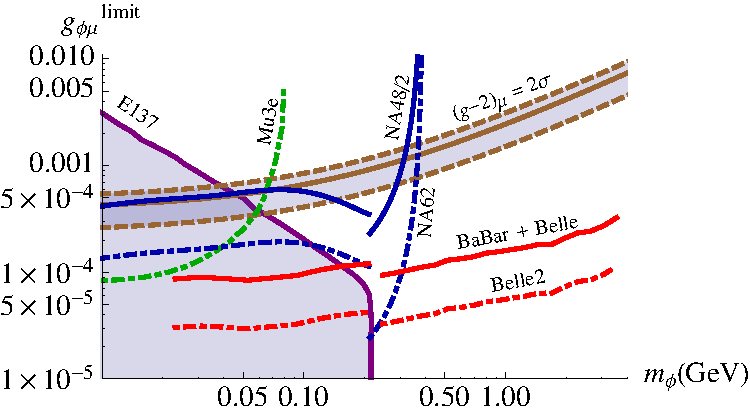
\includegraphics[width=0.9\textwidth]{Figures/limits/best_limits}
    \caption[Collection of the most promising sensitivity projections found in this work.]{Collection of the most promising sensitivity projections found in this work. Green shows the limits of phase II of \mueee, blue shows the NA48/2 and NA62 experiments, and red shows the combined \belle and \babar experiments, and \belletwo experiment. In purple are the constraints from the E137 beam dump experiment, as found in \cite{Batell:2015unpub}. Dot-dashed lines correspond to experiments not yet run, while solid lines correspond to data already taken. The band indicated by the brown and brown-dashed curves is the region where the $2\sigma$ anomaly of $(g-2)_\mu$ could be solved.} 
    \label{fig:best_limits}
\end{figure}

Utilizing the Monte Carlo generator \madgraph, we were able to phenomenologically explore the new scalar particle.
Restricting this particle to decay only to SM particles, in particular, pairs of leptons, allows one to put stringent bounds on the coupling, down to the level of $10^{-5}$ for the coupling to the muon.
Unlike the case of the dark photon that is thoroughly studied, much of the parameter space for the scalar remains unexplored.
A region of the currently allowed parameter space could serve as an explanation for the proton radius problem and the $(g-2)_\mu$ discrepancy.
Upcoming experiments offer a chance to test physics at the intensity frontier where many decays and collisions take place, allowing restrictions on branching ratios of SM physics to be placed down to the level of $10^{-16}$ in coming years.
The data collected from these experiments will be used to test this model and many other low mass theories.
The sensitivity limits placed were on the experiments \mueee, NA48/2, NA62, \babar, \belle, and \belletwo, across a large mass range from $2m_e$ up to $2m_\tau$.

There is also a large amount of future work that can be performed by the experimental collaborations to obtain a more accurate representation of the upper limits at these experiments.
First, a more robust treatment of the detectors would be a sensible way to proceed.
Most experiments likely have a \geant model that would be useful in these scenarios.
At the very least, performing Monte Carlo to find the signal efficiencies and mass resolution with these models would bear the most fruit, as these are hard to estimate without a robust Monte Carlo code.
Currently we use the condition that $S = 3\sqrt{B}$ for sensitivity in most cases, and then examine a signal bin; this could be improved with a proper likelihood fit or by utilizing a Feldman-Cousins technique.
However, doing this has diminishing returns since we are merely projecting expected limits and not actively searching for any.
In the B-factory cases, it is also possible to go beyond $2m_\tau$ if we consider a signal with muons in the final state instead of taus.
Variants on the model can also be discussed.
We may attempt to put a pseudo-scalar into the model, or examine the vector or axial-vector cases, or even simply play with the coupling strength being proportional to the lepton masses.
Finally, more experiments are being pursued that may be able to shine light on portions of the parameter space.
Fermilab will soon have a new measurement of $(g-2)_\mu$, and the proton charge radius with muons will be studied by scattering muons off of protons at \muse.
Other experiments such as \mutoe~\cite{Abrams:2012er} or \comet~\cite{Cui:2009zz} could similarly play an important role when examining lepton flavour violation in the charged lepton sector.
We conclude by noting that there is the possibility for this model to be tested rigorously and the parameter space explored over the next few years by many experiments, some of which were discussed in detail in this thesis.
